%% REPLACE sXXXXXXX with your student number
\def\studentNumber{S2569758}


%% START of YOUR ANSWERS
%% Add answers to the questions below, by replacing the text inside the brackets {} for \youranswer{ "Text to be replaced with your answer." }. 
%
% Do not delete the commands for adding figures and tables. Instead fill in the missing values with your experiment results, and replace the images with your own respective figures.
%
% You can generally delete the placeholder text, such as for example the text "Question Figure 3 - Replace the images ..." 
%
% There are 5 TEXT QUESTIONS. Replace the text inside the brackets of the command \youranswer with your answer to the question.
%
% There are also 3 "questions" to replace some placeholder FIGURES with your own, and 1 "question" asking you to fill in the missing entries in the TABLE provided. 
%
% NOTE! that questions are ordered by the order of appearance of their answers in the text, and not necessarily by the order you should tackle them. You should attempt to fill in the TABLE and FIGURES before discussing the results presented there. 
%
% NOTE! If for some reason you do not manage to produce results for some FIGURES and the TABLE, then you can get partial marks by discussing your expectations of the results in the relevant TEXT QUESTIONS. The TABLE specifically has enough information in it already for you to draw meaningful conclusions.
%
% Please refer to the coursework specification for more details.


%% - - - - - - - - - - - - TEXT QUESTIONS - - - - - - - - - - - - 

 % ----------------------------- Question 1: ----------------------------- %
\newcommand{\questionOne} {
\youranswer{From Figure 2 and 3, we can see that there is a healthy amount of gradient flow across the different layers of VGG 08 model, but not the VGG 38 model. This indicates that the gradient is not flowing properly through the layers of the VGG 38 model pointing that it suffers from a vanishing gradient problem which is hampering the training of the model. 
This is further supported by Figure 1 (a) and (b) which show that the loss of the VGG 38 model remains high while the accuracy being very low on both the training and the validation datasets.}
}
% Question 1 - Use Figures 1, 2, and 3 to identify the Vanishing Gradient Problem (which of these model suffers from it, and what are the consequences depicted?).
% The average length for an answer to this question is approximately 1/5 of the columns in a 2-column page

% ----------------------------- Question 2: ----------------------------- %
\newcommand{\questionTwo} {
\youranswer{A complex model like VGG38 has a lot of network capacity due to its deeper architecture. But a complex model like this is more likely to encounter the vanishing gradients problem, hindering effective weight update in its earlier layers (Figure 3). This is too be observed because VGG38 has an exteremly deep architecture and is made to handle more complex 
tasks and larger datasets. The image size of the CIFAR100 class is only $32\times32$ with 100 classes which is very less for VGG38. In contrast, a shallower model with relatively less network capacity (VGG08), exhibits normal gradient flow and is able to use its architecture and depth more efficiently to learn the data and train a relatively better model.
Some other factors that may have contributed to this difference include the model architecture, optimisation techniques used and the quality of the dataset.}
}
% Question 2 - Consider these results (including Figure 1 from \cite{he2016deep}). Discuss the relation between network capacity and overfitting, and whether, and how, this is reflected on these results. What other factors may have lead to this difference in performance?
% The average length for an answer to this question is approximately 1/5 of the columns in a 2-column page}

% ----------------------------- Question 3: ----------------------------- %
\newcommand{\questionThree} {
\youranswer{Residual connections are difficult to implement in downsampling layers because of the mismatch in the dimension from the residual to the point where it is being added back to the network. We would have to alter the model architecture in order to incorportate this ability in our model. This residual connection would serve as a shortcut for the gradients to 
directly flow through, skipping layers and preserving the gradient information helping in better training of deep models. There are 2 primary ways to implement this - Direct Residual Connections \& Bottleneck Residual Connections \cite{he2016deep}:
\begin{itemize}
    \item Direct Residual Connections: In this method, the input gradients are directly added to the output of the downsampled layer. This method is very intuitive and relatively easy to implement in the model architecture. If we were to look at the downsides of this method, it still carries the risk of attracting the phenomenon of vanishing gradients in very deep models. 
    It might also be not very efficient for models with extensive depth.
    \item Bottleneck Residual Connections: This method utilises $1\times1$ convolutions to reduce and expand the number of features in the model enabling healthier gradient flow. This also helps in reducing the number of parameters effectively reducing the computational cost of the model. Although it is better at tackling the issue of vanishing gradients in very deep models, 
    it is more complex than Direct Residual Connections and adds extra $1\times1$ convolutions to the model architecture.
\end{itemize}}
}
% In this coursework, we didn't incorporate residual connections to the downsampling layers. Explain and justify what would need to be changed in order to add residual connections to the downsampling layers. Give and explain 2 ways of incorporating these changes and discuss pros and cons of each.

% ----------------------------- Question 4: ----------------------------- %
\newcommand{\questionFour} {
\youranswer{Variety of experiments were performed on the VGG38 model implementing a plethora of techniques to combat the vanishing gradient problem and then check its performance on the CIFAR100 dataset. A baseline VGG08 model was used a reference point which did not suffer from a vanishing gradient problem like the baseline VGG38 model did.\par

We introduced batch normalisation and residual connections in the VGG38 model architecture to combat the problem of vanishing gradients. Batch Normalisation prevents the weights from getting too large or small ensuring a healthy flow of the gradient through the layers. It is to be noted that the addition of Batch Normalisation adds approximately \textit{3,000} parameters to the 
model increasing the computational cost to train it. Direct Residual Connections (Section 5.1) does not add any parameters to the model. It ensures the preservation of gradient in training of very deep models.\par 

The introduction of these modifications instantly fixes the problem of vanishing gradient and the model starts to learn some features from the data. Keeping the learning rate constant, the end results are marginally better than that of the baseline VGG08 model but the loss is still relatively high and there is still room for improvement in the accuracy of the model (Table 1).\par

We then combined the two methods to see if they boost the model performance. There was little improvement when compared to the model with residual connections indicating that other parameters of the model have to be changed to get better results. The learning rate (LR) was increased to \textit{0.01} from \textit{0.001}. This was first changed in the model with only batch 
normalisation to study its effects on the model. This variation ended up performing worse than the previous models (Table 1). \par

This new learning rate was then applied to the VGG38 model with both Batch Normalisation and Residual Connections. This significantly improved the model's performance on the train set but not that much test set. This combination of large learning rate with BN and RC has ensured the healthy flow of gradient, but due to its huge network capacity and small 
dataset for its size, the model is still overfitting on the data.\par

Taking this experiment further, we can try modifying the LR in the VGG38 model with just RC and see how the relatively big jumps in gradients are influenced by shortcuts in the different layers of the CNN.}
}
% Question 4 - Present and discuss the experiment results (all of the results and not just the ones you had to fill in) in Table 1 and Figures 4 and 5 (you may use any of the other Figures if you think they are relevant to your analysis). You will have to determine what data are relevant to the discussion, and what information can be extracted from it. 
% Also, discuss what further experiments you would have ran on any combination of VGG08, VGG38, BN, RC in order to
% - Improve performance of the model trained (explain why you expect your suggested experiments will help with this).
% - Learn more about the behaviour of BN and RC (explain what you are trying to learn and how).
% The average length for an answer to this question is approximately 1 of the columns in a 2-column page

% The next step was to introduce Residual Connections in the VGG38 model. These shortcuts preserve the gradient and help in the training of very deep models like the VGG38. This is again proven to be an effective method for tackling vanishing gradients and lets the model learn features of the dataset. As discussed in Section 5.1, there are different ways to implement residual 
% connection in a model architecture. We have used direct residual connection methodolgy for this experiment which does not add any parameters to the model. The performance of this version of VGG38 is only marginally better than the VGG38 model with batch normalisation (Table 1).\par
% WRITE ABOUT OTHER EXPERIMENTS TO RUN WHICH WILL IMPROVE THE MODEL OR HOW WE CAN LEARN FROM BN \& RC. \\
% TALK ABOUT FIXING THE MODEL WITH BOTH BN AND RC TOGETHER}

% ----------------------------- Question 5: ----------------------------- %
\newcommand{\questionFive} {
\youranswer{Question 5 - Briefly draw your conclusions based on the results from the previous sections (what are the take-away messages?) and conclude your report with a recommendation for future work. 

Good recommendations for future work also draw on the broader literature (the papers already referenced are good starting points). Great recommendations for future work are not just incremental (an example of an incremental suggestion would be: ``we could also train with different learning rates'') but instead also identify meaningful questions or, in other words, questions with answers that might be somewhat more generally applicable. 

For example, \citep{huang2017densely} end with \begin{quote}``Because of their compact internal representations and reduced feature redundancy, DenseNets may be good feature extractors for various computer vision tasks that build on convolutional features, e.g.,  [4,5].''\end{quote} 

while \cite{bengio1993problem} state in their conclusions that \begin{quote}``There remains theoretical questions to be considered,  such as whether the problem with simple gradient descent  discussed in this paper would be observed with  chaotic attractors that are not  hyperbolic.''\\\end{quote}

The length of this question description is indicative of the average length of a conclusion section}
}


%% - - - - - - - - - - - - FIGURES - - - - - - - - - - - - 

%% Question Figure 3:
\newcommand{\questionFigureThree} {
\youranswer{Question Figure 3
% \textit{(The provided figure is correct, and can be used in your analysis. It is partially obscured so you can get credit for producing your own copy).}
\begin{figure}[t]
    \centering
    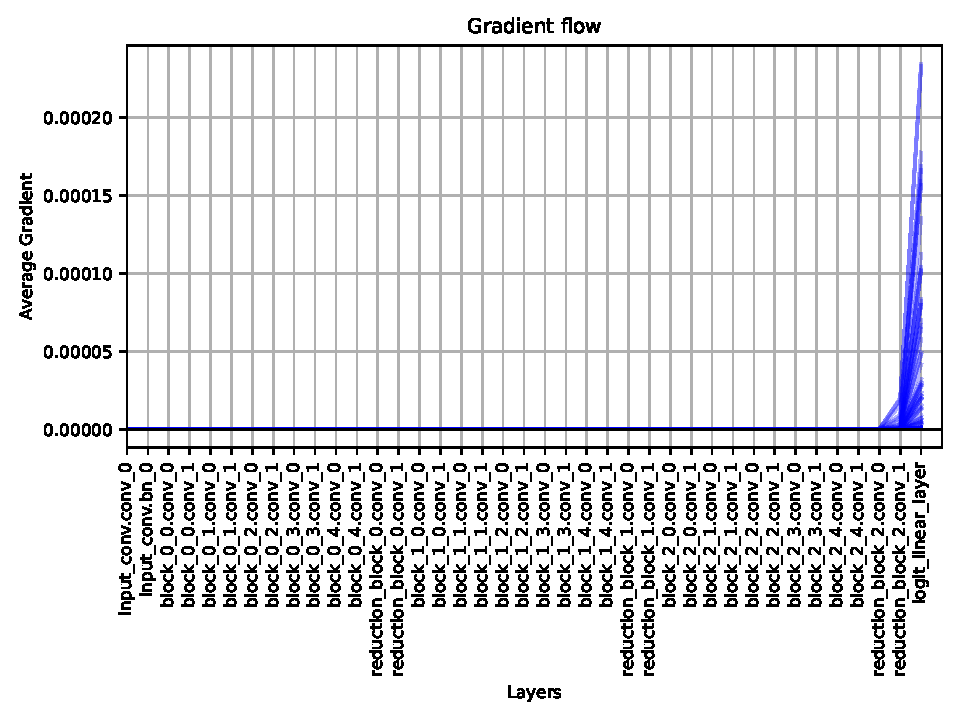
\includegraphics[width=\linewidth]{figures/vgg38_gf_bl.pdf}
    \caption{Gradient Flow on VGG38}
    \label{fig:grad_flow_38}
\end{figure}
}}

%% Question Figure 4:
\newcommand{\questionFigureFour} {
\youranswer{Question Figure 4
% Replace this image with a figure depicting the training curves for the model with the best performance \textit{across experiments you have available (you don't need to run the experiments for the models we already give you results for)}. Edit the caption so that it clearly identifies the model and what is depicted.
\begin{figure}[t]
    \centering
    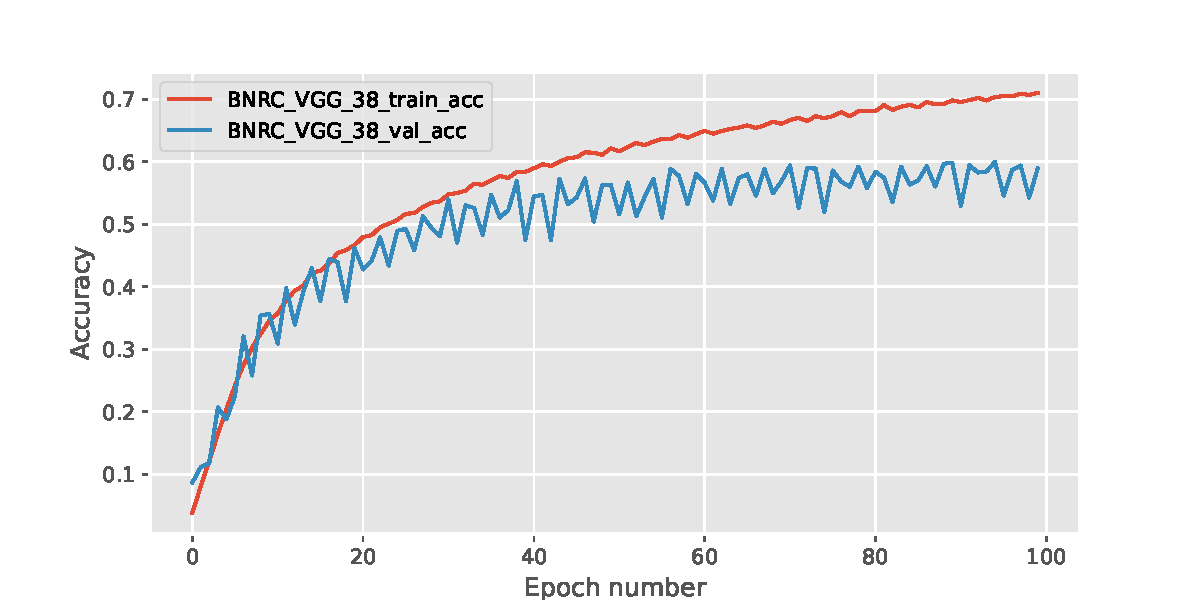
\includegraphics[width=\linewidth]{figures/best_model_accuracy_performance.pdf} % Placeholder - example-image-duck
    \caption{Training curves for VGG38 with Batch Normalisation and Residual Connections in terms of classification accuracy}
    \label{fig:grad_flow_bestModel}
\end{figure}
}}

%% Question Figure 5:
\newcommand{\questionFigureFive} {
\youranswer{Question Figure 5
% Replace this image with a figure depicting the average gradient across layers, for the model with the best performance \textit{across experiments you have available (you don't need to run the experiments for the models we already give you results for)}. Edit the caption so that it clearly identifies the model and what is depicted.
\begin{figure}[t]
    \centering
    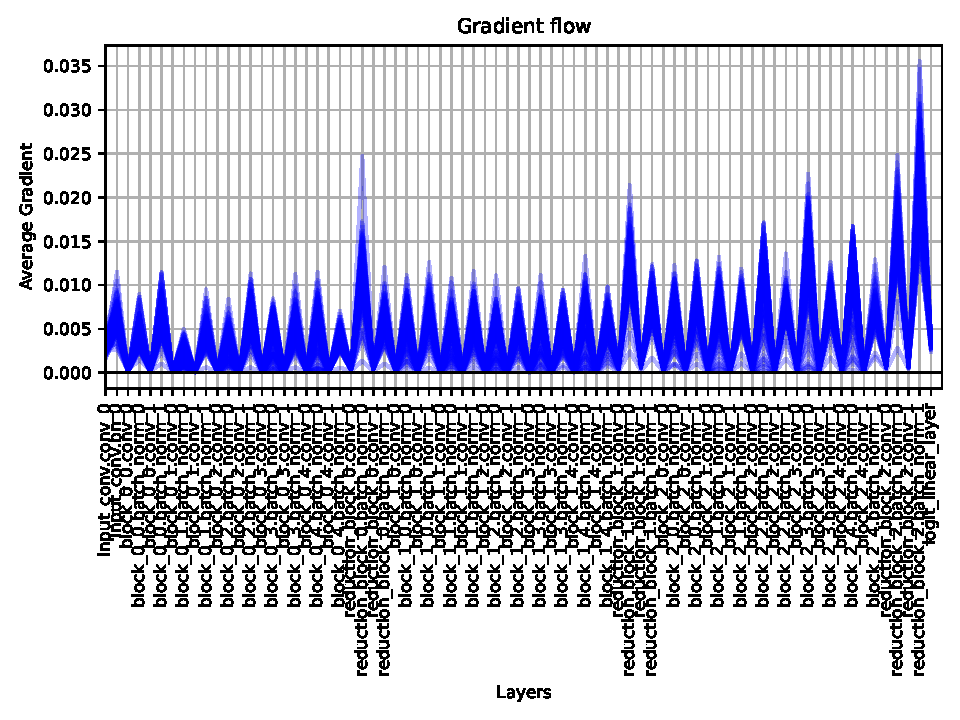
\includegraphics[width=\linewidth]{figures/vgg38_bnrc_gf.pdf} % Placeholder - example-image-duck
    \caption{Gradient Flow on VGG38 with Batch Normalisation and Residual Connections}
    \label{fig:grad_flow_bestModel}
\end{figure}
}}

%% - - - - - - - - - - - - TABLES - - - - - - - - - - - - 

%% Question Table 1:
\newcommand{\questionTableOne} {
\youranswer{Question Table 1:\par \textit{VGG38 BN (LR 1e-3)} and \textit{VGG38 BN + RC (LR 1e-2)}.
% Fill in Table 1 with the results from your experiments on 
\begin{table*}[t]
    \centering
    \begin{tabular}{lr|ccccc}
    \toprule
        Model                   & LR   & \# Params & Train loss & Train acc & Val loss & Val acc \\
    \midrule
        VGG08                   & 1e-3 & 60 K      &  1.74      & 51.59     & 1.95     & 46.84 \\
        VGG38                   & 1e-3 & 336 K     &  4.61      & 00.01     & 4.61     & 00.01 \\
        VGG38 BN                & 1e-3 & 339 K     &  1.65      & 53.33     & 1.86     & 48.60 \\
        VGG38 RC                & 1e-3 & 336 K     &  1.33      & 61.52     & 1.84     & 52.32 \\
        VGG38 BN + RC           & 1e-3 & 339 K     &  1.26      & 62.99     & 1.73     & 53.76 \\
        VGG38 BN                & 1e-2 & 339 K     &  1.70      & 52.28     & 1.99     & 46.72 \\
        VGG38 BN + RC           & 1e-2 & 339 K     &  0.96      & 71.01     & 1.63     & 58.96 \\
    \bottomrule
    \end{tabular}
    \caption{Experiment results (number of model parameters, Training and Validation loss and accuracy) for different combinations of VGG08, VGG38, Batch Normalisation (BN), and Residual Connections (RC), LR is learning rate.}
    \label{tab:CIFAR_results}
\end{table*} 
}
}

%% END of YOUR ANSWERS
